\section{Dual-Task Learning Program Repair}
\label{sec: dual-learning}
\begin{figure}[t]
	\centering
	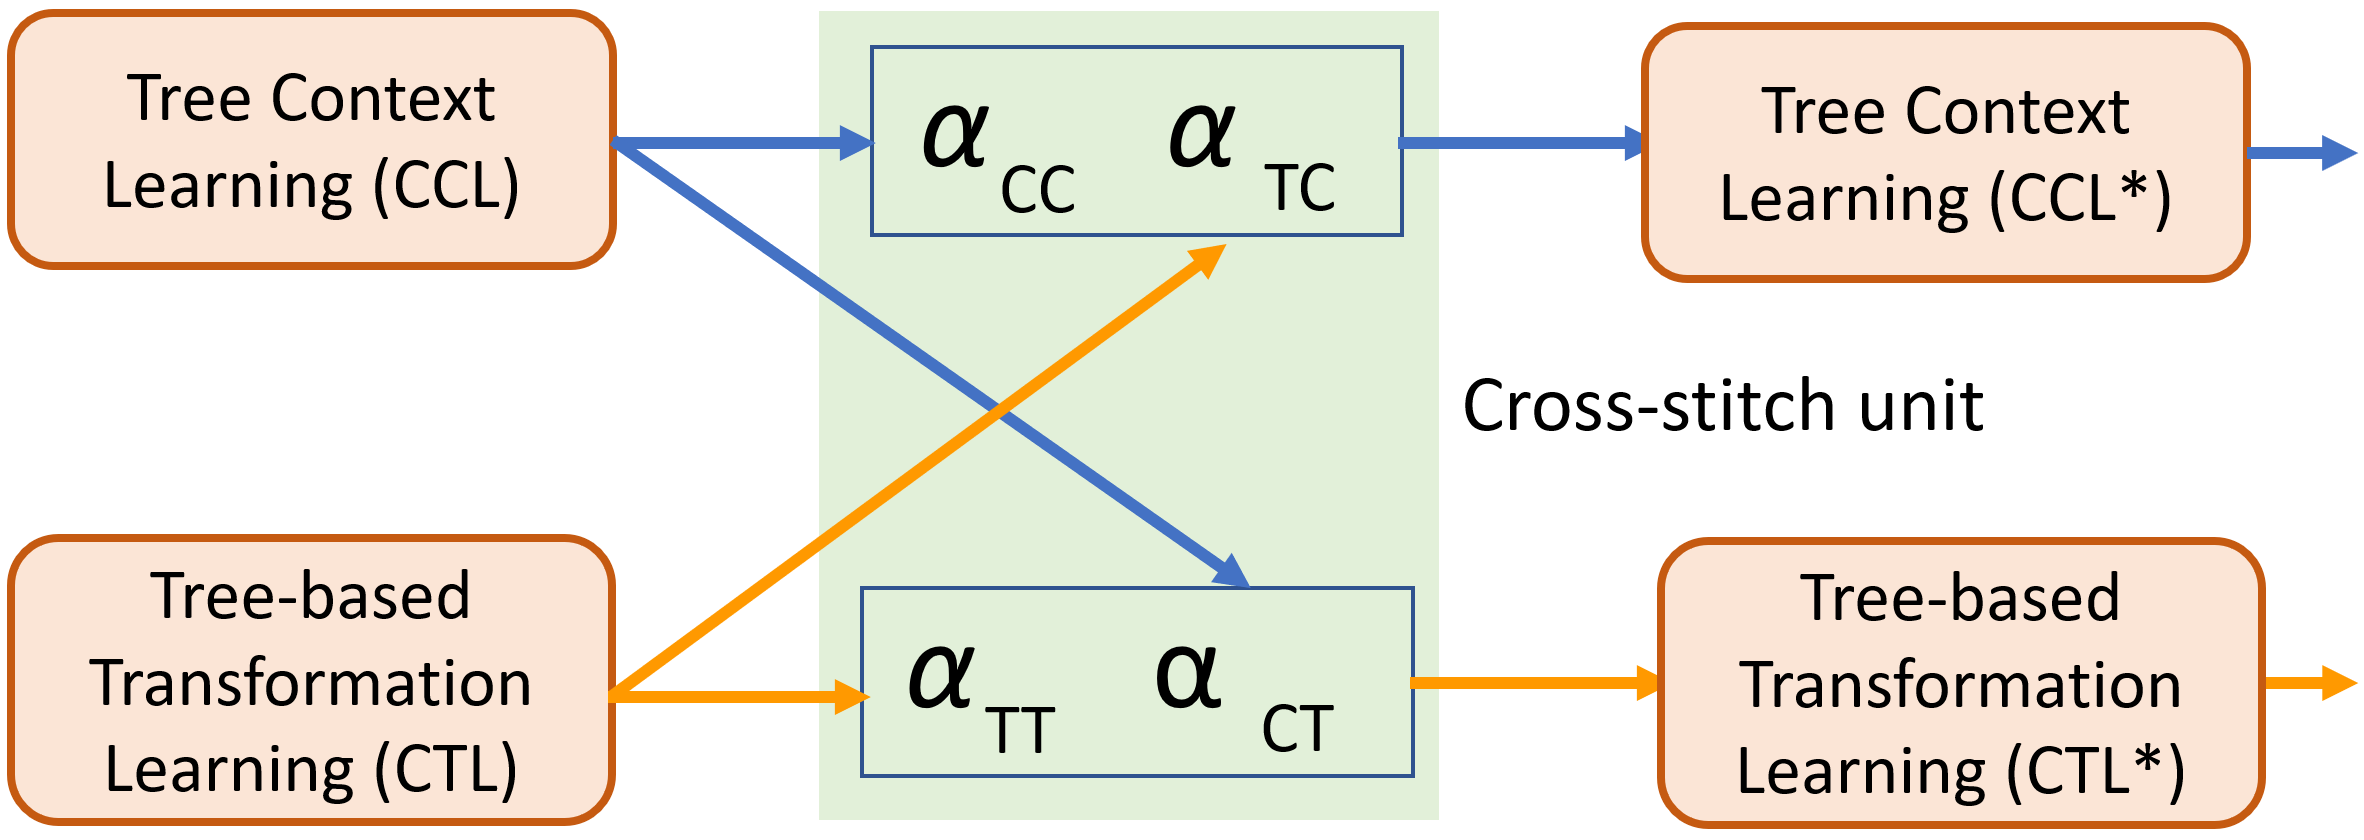
\includegraphics[width=3in]{graphs/cross-stitch}
        \vspace{-9pt}
	\caption{Cross-Stitch Unit for Joint Training~\cite{misra2016cross}}
	\label{fig:cross-stitch}
\end{figure}

After the representation learning step, we obtain the vectorized AST
$T^{M}_b$ for the buggy method $M$ and the vectorized AST subtree
$T^{s}_b$ for the buggy statement $s$, as well as the one for the
respective fixed method $T^{M}_f$ and the one for the respective fixed
statement $T^{s}_f$. $T^{M}_b$ and $T^{M}_f$ are used at the input and
output layers of CCL; and $T^{s}_b$ and $T^{s}_f$ are used at the
input and output layers of CTL.
%Let us explain the dual-task learning framework for CCL and CTL.

%After having the $Tree_m$, $Tree_{mf}$ pair and $Tree_s$, $Tree_{sf}$ pair from the first step, \tool uses them as the input and the ground truth to train the dual learning program repair model in this step. \tool uses the generated after fixing AST $Tree'_m$ and after fixing subtree of AST $Tree'_s$ as output for this step when making the prediction. Specifically, there are two small steps, including the AST node representation learning and the dual learning framework.


\subsection{Cross-Stitch Unit}

We perform a joint training between CCL and CTL via a cross-stitch
unit~\cite{misra2016cross}. Let us first explain the cross-stitch unit
and then how we leverage it for the Automated Program Repair problem.



In Figure~\ref{fig:cross-stitch}, for dual-task learning, we use the
cross-stitch unit to connect CCL and CTL. The sharing of
representations between CCL and CTL is modeled by the learning a
linear combination of the input features from the vectorized AST
(sub)trees. The top output of the cross-stitch unit, which becomes
CCL*, gets direct supervision from CCL and indirect supervision from
CTL. Cross-stitch units help regularize both CCL and CTL by learning
and enforcing shared representations by combining feature
maps~\cite{misra2016cross}.

The goal of a cross-stitch unit is to learn a linear combination of
both inputs from CCL and CTL, which are parameterized
using the weights $\alpha$. The output of the cross-stitch unit is
computed as:
\begin{equation}\label{eq:cross-stitch}
	\begin{bmatrix}
		O_C\\
		O_T
	\end{bmatrix}
	=
	\begin{bmatrix}
		\alpha_{CC} &  \alpha_{CT} \\
		\alpha_{TC} &  \alpha_{TT}
	\end{bmatrix}
	\begin{bmatrix}
		I_C\\
		I_T
	\end{bmatrix}
\end{equation}
$I_C$ and $I_T$ are the inputs for the cross-stitch unit, which are
the outputs from a layer of CCL and CTL. $O_C$ and $O_T$ are the
outputs from the cross-stitch unit, which can be used as the inputs
for the next layer of the two models. In this case, the next layers
(noted as CCL* and CTL*) are the ones with the shared representations
and having the joint training. More details on cross-stitch are
in~\cite{misra2016cross}.

\subsection{Tree-based, Dual-Task Learning}

\begin{figure}[t]
	\centering
	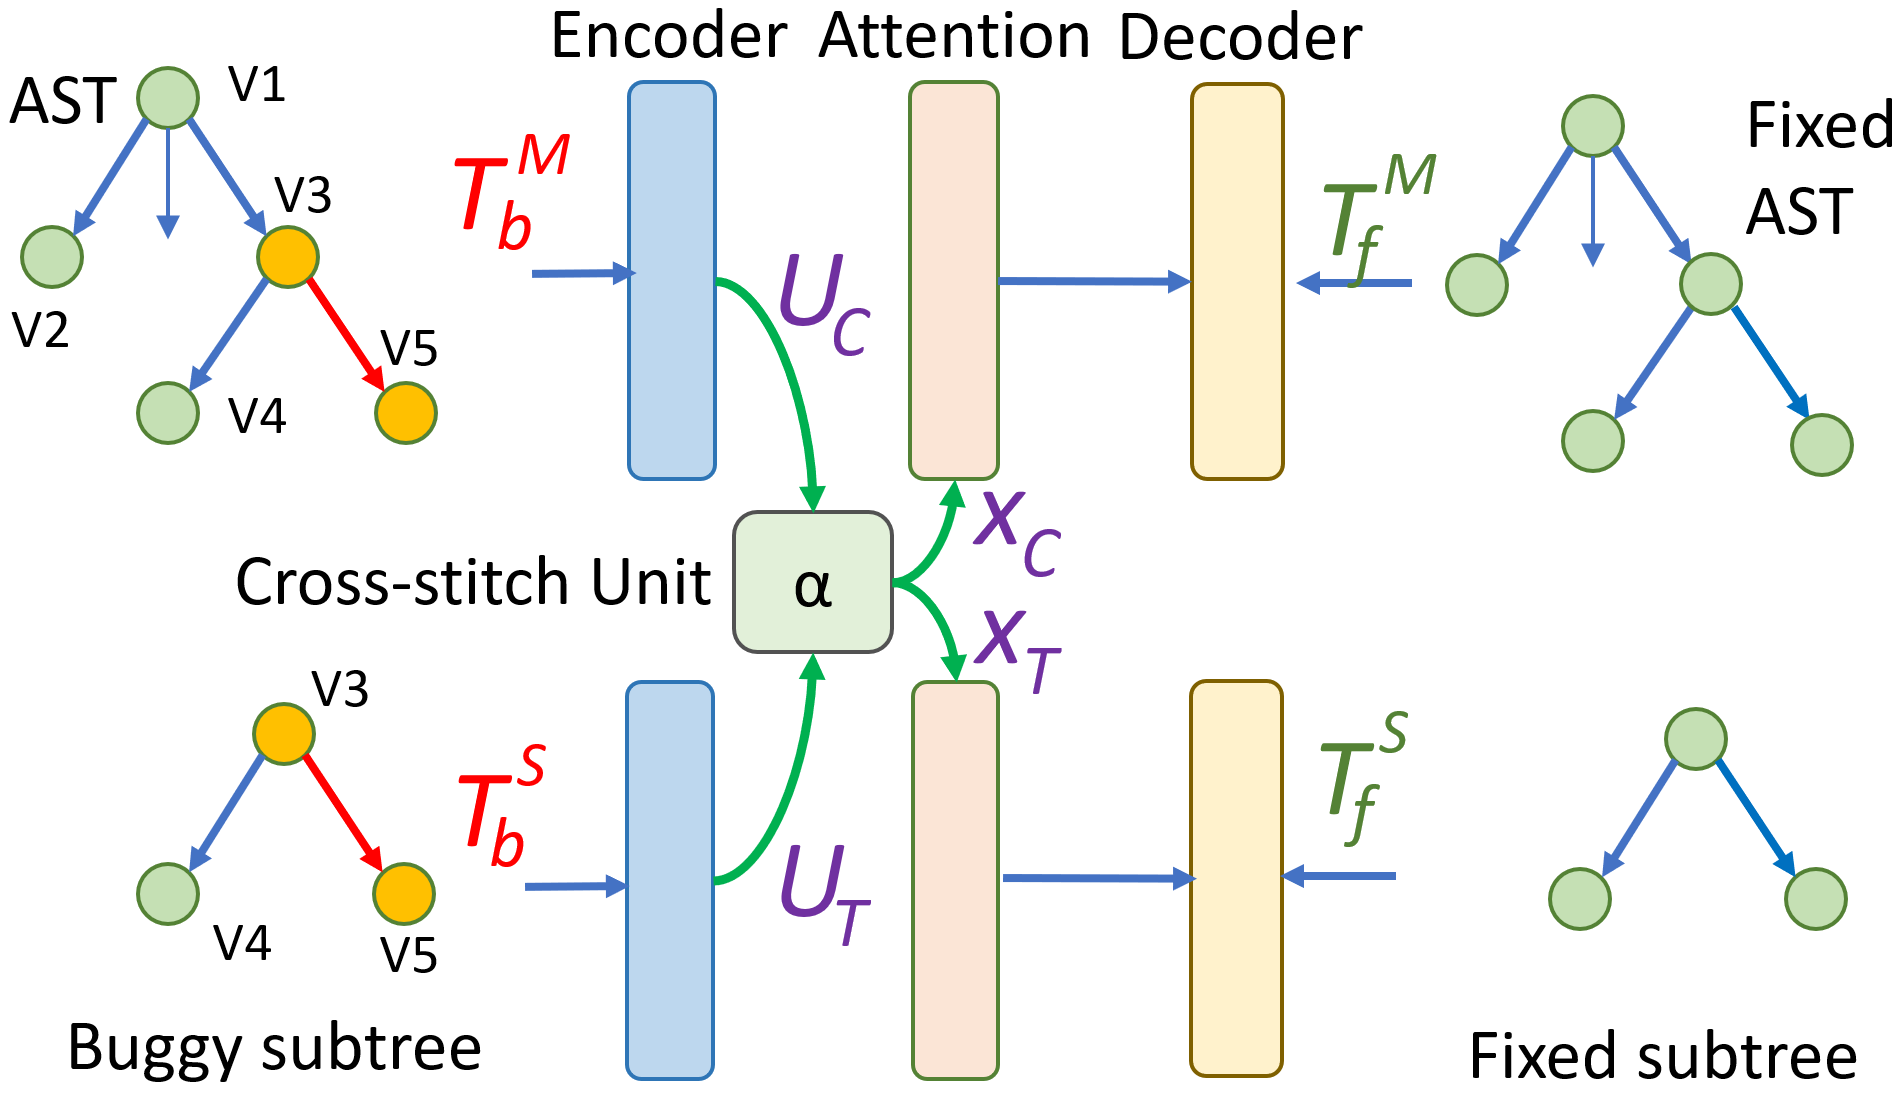
\includegraphics[width=2.8in]{graphs/dual-learning-repair.png}
        \vspace{-9pt}
	\caption{Dual-Task Learning between CCL and CTL}
	\label{fig:dual-learning}
\end{figure}

We have modified cross-stitch unit to work with AST representations as
follows (Figure~\ref{fig:dual-learning}). We use two separate
attention-based \code{seq2seq} models for CCL and CTL.
%The dual-task training is shown in Figure~\ref{fig:dual-learning}.
We use TreeCaps~\cite{bui2021treecaps} with an attention layer in
between of an encoder and a decoder. In a regular attention-based
\code{seq2seq} model, the hidden state output from the encoder is
directly connected to the attention layer. In {\tool}, we use a
cross-stitch unit to accept as the input the hidden states from the
outputs of the encoders of CCL and CTL. The outputs of the
cross-stitch units are connected to the attention layers of both the
models. This joint training enables propagating the mutual
impact of context learning and transformation learning in both
directions.

\subsubsection*{\bf Formulation.}
As we use TreeCaps~\cite{bui2021treecaps}, which is built on top of
$k$ TBCNN layers~\cite{mou2014tbcnn}, at the $k^{th}$ layer, the
output of the convolution window is calculated as:
\begin{equation}\label{eq:treecaps}
	Y = tanh(\sum_{i=1}^{N}[\Delta^t_iW^t + \Delta^t_iW^t + \Delta^t_iW^t]X_i + b)
\end{equation}
Where $\Delta$ are the weights calculated corresponding to the depth
and the position of the nodes in a tree. This is the mechanism in
TreeCaps to learn the importance of the position of a node in a
tree. $W$ is the trainable matrix; $b$ is the bias factor; $N$ is the
total number of nodes in the convolution window. TreeCaps merges the
output from all TBCNN layers by using a non-linear squash
function~\cite{sabour2017dynamic}. For an AST node $j$, TreeCaps
calculates the capsule $u_j$ as follows (Details of the computation of
$Y$ and $u_j$ can be found in~\cite{bui2021treecaps}):
\begin{equation}\label{eq:2}
	u_j = \frac{||c_j||^2}{||c_j||^2+1}\frac{c_j}{||c_j||}
\end{equation}
We then perform a depth-first-search traversal, and merge all the
capsules of all the nodes in that order. We consider the list of
capsules as the output $U$ of the TreeCaps model. With both
CCL and CTL, we have the outputs $U_C$ for the context
learning part and $U_T$ for the transformation learning part.

With both $U_C$ and $U_T$ as the inputs of the cross-stitch unit, the
outputs of the cross-stitch unit are computed as:
\begin{equation}\label{eq:3}
	\begin{bmatrix}
		X_C\\
		X_T
	\end{bmatrix}
	=
	\begin{bmatrix}
		\alpha_{CC} &  \alpha_{CT} \\
		\alpha_{TC} &  \alpha_{TT}
	\end{bmatrix}
	\begin{bmatrix}
		U_C\\
		U_T
	\end{bmatrix}
\end{equation}
Where $\alpha$ is the trainable weight matrix, $X_C$ and $X_T$ are the
outputs of the cross-stitch unit, which are in turn fed into the
attention layers of both models. $X_C$ and $X_T$ contain the
information learned from both context learning and transformation
learning models, which helps achieve the main goal of dual-task learning
to enhance the APR performance. From Formula~\ref{eq:3}, we have
\begin{equation}\label{eq:4}
	X_C = \alpha_{CC}U_C + \alpha_{CT}U_T
\end{equation}
\begin{equation}\label{eq:5}
	X_T = \alpha_{TC}U_C + \alpha_{TT}U_T
\end{equation}
If the $X_C$ and $X_T$ have different sizes, we need to resize them
for consistence. If the size needs to be increased, we use bilinear
interpolation~\cite{bilinear-interpolation} for resizing. If the size
needs to be reduced, we do the center crop on the matrix to match the
required size. Moreover, for efficiency, we also have a size limit for
the fixed tree in which each buggy tree has at most $P+P^2+...+P^Q$
nodes.  $P$ is the max number of children nodes of a node and $Q$ is
the max child node depth. When predicting, if one vector is close
to zero, we consider it as empty, and all of its children nodes are
considered as empty.

%After solving this, here is one last problem the dual learning may
%face. When making the prediction, because we don't know how the tree
%structure changes, \tool needs to have a size limit to control the
%fixing. \tool expands the child node number to $P$ and expands the
%child node depth to $Q$ for a buggy node. It means that we make each
%buggy node have at most $P+P^2+...+P^Q$ nodes.
%When making predictions, if one vector is close to zero, we consider
%it as empty, and all of its children nodes are considered as empty.

%First, \tool uses two separate attention-based seq2seq frameworks to learn the code fixing for both the method-level and the statement-level. We all use the tree-based deep learning model to process the AST or subtree of AST for the encoder and decoder of these two tasks. Based on the recent study, we select a well-performed baseline TreeCaps \cite{bui2021treecaps} here to do so. Between the encoder and decoder, there is an attention layer for both tasks to help improve the accuracy of generating the fixing.

%In the regular attention-based seq2seq model, the hidden status $H$ is directly passed to the attention layer. However, \tool uses a cross-stitch unit to accept the hidden status $H_m$ and $H_s$ from both method-level and the statement-level to achieve the dual learning. And then, the \tool passes the output of the cross-stitch unit to the method-level and statement-level attention layer. Just like the Figure \ref{program-repair} shown, the output from the encoder does not go to the attention layer. They go to the cross-stitch unit instead. The cross-stitch unit helps both the method-level and the statement-level attention-based seq2seq model catch the input features within the buggy method and the buggy statement.



%As for the TreeCaps model \tool is using, it is built on top of $k$
%TBCNN layers \cite{mou2014tbcnn}. So, for the TBCNN layer $k$, the
%output of the convolution window is calculated as:





%After \tool has $H_m$ and $H_s$ for both method-level and
%statement-level in the encoder, we aim to learn the linear
%combinations of both inputs of the cross-stitch unit. The output of
%the cross-stitch unit is computed as:







%After solving this, here is one last problem the dual learning may face. When making the prediction, because we don't know how the tree structure changes, \tool needs to have a size limit to control the fixing. \tool expands the child node number to $P$ and expands the child node depth to $Q$ for a buggy node. It means that we make each buggy node have at most $P+P^2+...+P^Q$ nodes. When making predictions, if one node is close to zero, we think it is empty and drop it. At the same time, all child nodes of it will be dropped by \tool.
